\documentclass[11pt]{elegantbook}
\definecolor{structurecolor}{RGB}{40,58,129}
\linespread{1.6}
\setlength{\footskip}{20pt}
\setlength{\parindent}{0pt}
\newcommand{\argmax}{\operatornamewithlimits{argmax}}
\newcommand{\argmin}{\operatornamewithlimits{argmin}}
\elegantnewtheorem{proof}{Proof}{}{Proof}
\elegantnewtheorem{claim}{Claim}{prostyle}{Claim}
\DeclareMathOperator{\col}{col}
\title{\textbf{Linear Algebra}}
\author{Wenxiao Yang}
\institute{University of Illinois at Urbana-Champaign; University of California Berkeley}
\date{2023 (Last Updated)}
\setcounter{tocdepth}{2}
\cover{cover.jpg}
\extrainfo{All models are wrong, but some are useful.}

% modify the color in the middle of titlepage
\definecolor{customcolor}{RGB}{32,178,170}
\colorlet{coverlinecolor}{customcolor}
\usepackage{cprotect}

\addbibresource[location=local]{reference.bib} % bib

\begin{document}

\maketitle
\frontmatter
\tableofcontents
\mainmatter


\chapter{Field and Vector Space}
\section{Field $(\mathbb{F},+,\cdot)$}
\subsection{Definition of Field \small{(@ Lec 02 of ECON 204)}}
\begin{definition}[Field]
    \normalfont
    A \textbf{field} $\mathcal{F}=(\mathbb{F},+,\cdot)$ is a 3-tuple consisting of a set $\mathbb{F}$ and two binary operations $+,\cdot: \mathbb{F}\times \mathbb{F} \rightarrow \mathbb{F}$ such that
    \begin{enumerate}
        \item $+$ is associative, commutative.
        \item Exists (unique) additive identity and (unique) additive inverse.
        \item $\cdot$ is associative, commutative.
        \item Exists (unique) multiplicative identity and (unique) multiplicative inverse.
        \item Distributivity of multiplication over addition.
    \end{enumerate}
\end{definition}

\begin{example}[ of Field]
    \begin{enumerate}
        \item $\mathbb{R}$, $\mathbb{C}$, $\mathbb{Q}$ are field;
        \item $\mathbb{N}$, $\mathbb{Z}$ are not field;
        \item $\mathbb{Q}(\sqrt{2})=\{q+r\sqrt{2}: q,r\in \mathbb{Q}\}$ is the smallest filed containing $\mathbb{Q}\cup \sqrt{2}$.
    \end{enumerate}
\end{example}

\section{Vector Space}
\subsection{Definition of Vector Space \small{(@ Lec 02 of ECON 204)}}
\begin{definition}[Vector Space]
    \normalfont
    A \underline{vector space} over a field $\mathbb{F}$, $(V, \mathbb{F}, +,\times)$, is a set $V$ w/ an operation \underline{addition} $+ : V \times V \rightarrow V$ and an operation \underline{scalar multiplication} $\mathbb{F} \times V \rightarrow V$
    \begin{enumerate}
        \item $+$ is associative, commutative.
        \item Exists (unique) additive identity and (unique) additive inverse.
        \item $\cdot$ is associative (there is no need to consider commutativity).
        \item Exists (unique) multiplicative identity (there is no need to consider inverse).
        \item Distributivity of scalar multiplication over vector addition: $\forall \alpha\in\mathbb{F},\ v,u\in V,\ \alpha(v+u)=\alpha v+\alpha u$
        \item Distributivity of scalar multiplication over scalar addition: $\forall \alpha,\beta\in\mathbb{F},\ v\in V,\ (\alpha+\beta)v=\alpha v+\beta v$
    \end{enumerate}
\end{definition}
We often say “$V$ is a vector space over $\mathbb{F}$”.

\begin{example}
    \begin{enumerate}
        \item $\mathbb{R}^n$ is a vector space over $\mathbb{R}$, for any $n\in \mathbb{N}$.
        \item $\mathbb{Q}(\sqrt{2})$ is a vector space over $\mathbb{Q}$. (It is $\mathbb{Q}^2$, using $(q,r)$ versus $q+r\sqrt{2}$).
        \item $\mathbb{Q}(\sqrt[3]{2})$ is a vector space over $\mathbb{Q}$. (It is $\mathbb{Q}^3$, using $(q,r,v)$ versus $q+r 2^\frac{2}{3}+v2^\frac{1}{3}$).
        \item $C([0,1])$, the space of all continuous real-valued functions on $[0,1]$, is a vector space over $\mathbb{R}$.
    \end{enumerate}
\end{example}

\subsection{Theorem: A field is a vector space over its subfield}
\begin{theorem}
    $\mathbb{K}\subset\mathbb{F}$ is a subfield of a field $\mathbb{F}$. Then $\mathbb{F}$ is a vector space over $\mathbb{K}$.
\end{theorem}
\begin{example}
    Since $\mathbb{F}\subset \mathbb{F}[x]$, then $\mathbb{F}[x]$ is a vector space over $\mathbb{F}$.
\end{example}
\subsection{Vector Subspace}
Suppose that $V$ is a vector space over $\mathbb{F}$. A \underline{vector subspace} or just \underline{subspace} is a nonempty subset $W\subset V$ closed under addition and scalar multiplication. i.e. $v+w\in W,\ av\in W,\ \forall v,w\in W,\ a\in \mathbb{F}$.
\begin{example}
$\mathbb{K}\subset \mathbb{L}\subset \mathbb{F}$, then $\mathbb{L}$ is a subspace of $\mathbb{F}$ over $\mathbb{K}$.
\end{example}
\subsection{Linear independent, Linear combination}
\begin{definition}
    \normalfont
    A set $V \subseteq X$ is \textbf{linearly dependent} if there exist $v_1,...,v_n \in V$ and $\alpha_1,...,\alpha_n \in F$ not all zero such that $\sum_{i=1}^n\alpha_iv_i=0$.
\end{definition}

\subsection{span V, basis, dimension}
\begin{definition}[Span]
    \normalfont
    If $V \subseteq X$, the span of $V$, denoted $\textnormal{span }V$, is the set of all linear combinations of elements of $V$.

    The set $V \subseteq X$ \textbf{spans} $X$ if $\textnormal{span }V=X$.
\end{definition}

\begin{definition}[(Hamel) Basis]
    \normalfont
    A \textbf{Hamel basis} (often just called a \textbf{basis}) of a vector space $X$ is a \textbf{linearly independent} set of vectors in $X$ that \textbf{spans} $X$.
\end{definition}

\begin{proposition}[Proposition 2.4.10.]
    Suppose $V$ is a vector space over a field $\mathbb{F}$ having a basis $\{v_1,...,v_n\}$ with $n \geq 1$.
    \begin{enumerate}[(i).]
        \item For all $v \in V$ , $v = a_1 v_1 + ... + a_n v_n$ for exactly one $(a_1,...,a_n)\in \mathbb{F}^n$.
        \item If $w_1,...,w_n$ span $V$, then they are linearly independent.
        \item If $w_1,...,w_n$ are linearly independent, then they span $V$.
    \end{enumerate}
\end{proposition}
If a vector space $V$ over $\mathbb{F}$ has a basis with $n$ vectors, then $V$ is said to be n-dimensional (over $\mathbb{F}$) or is said to have \textbf{dimension} $n$.
\subsection{Standard basis vectors}
\begin{equation}
    \begin{aligned}
        e_1=(1,0,...,0),e_2=(0,1,0,...,0),...,e_n=(0,0,...,0,1)\in \mathbb{F}^n
    \end{aligned}
    \nonumber
\end{equation}
are a basis for $\mathbb{F}^n$ called the \textbf{standard basis vectors}.
\subsection{Linear transformation}
Given two vector spaces $V$ and $W$ over $\mathbb{F}$ a \textbf{linear transformation} is a function $T : V \rightarrow	 W$ such that
for all $a \in \mathbb{F}$ and $v,w \in V$ , we have
\begin{equation}
    \begin{aligned}
        T(av)=aT(v)\ and\ T(v+w)=T(v)+T(w)
    \end{aligned}
    \nonumber
\end{equation}
\begin{proposition}[Proposition 2.4.15.]
    If $V$ and $W$ are vector spaces and $v_1,...,v_n$ is a basis for $V$ then any function
    from $\{v_1,...,v_n\}\rightarrow W$ extends \textit{uniquely} to a linear transformation $V \rightarrow W$.
\end{proposition}
Any $v\in V$, $\exists (a_1,...,a_n)$ s.t. $v=a_1 v_1+...+a_n v_n$. Then $T(v)=T(a_1 v_1+...+a_n v_n)=a_1T(v_1)+...+a_nT(v_n)$\\
\subsection{A Linear Transformation Correponds to a Matrix}
\begin{corollary}[Corollary 2.4.16.]
    If $v_1,...,v_n$ is a basis for a vector space $V$ and $w_1,...,w_n$ is a basis for a vector space $W$ (both over $\mathbb{F}$), then any linear transformation $T : V \rightarrow W$ determines (and is determined by) the $m\times n$ matrix:
    \begin{equation}
        \begin{aligned}
            A=A(T)=\begin{bmatrix}
                A_{11}&	A_{12}&... &A_{1n}\\
                A_{21}&	A_{22}&... &A_{2n}\\
                \vdots&	\vdots&... &\vdots\\
                A_{m1}&	A_{m2}&... &A_{mn}
            \end{bmatrix}
        \end{aligned}
        \nonumber
    \end{equation}
\end{corollary}
\begin{equation}
    \begin{aligned}
        &\begin{bmatrix}
            w_1&\cdots	&w_m
        \end{bmatrix}^T=A
        &\begin{bmatrix}
                v_1&\cdots	&v_n
        \end{bmatrix}^T
    \end{aligned}
    \nonumber
\end{equation}
$\mathcal{L} (V,M)$ denotes the set of all linear transformations from $V$ to $W$; $M_{m\times n}(\mathbb{F})$ the set of $m\times n$ matrix with entries in $\mathbb{F}$. $T\rightarrow A(T)$ defines a \textit{bijection} $\mathcal{L} (V,M)\rightarrow M_{m\times n}(\mathbb{F})$. \textbf{$A(T)$ represents the linear transformation $T$}.


\begin{proposition}[Proposition 2.4.19]
    Suppose that $V$ , $W$, and $U$ are vector spaces over $\mathbb{F}$, with fixed chosen bases. If
    $T : V \rightarrow W$ and $S : W \rightarrow U$ are linear transformations represented by matrices $A = A(T)$ and $B = B(S)$,
    then $ST = S \circ T : V \rightarrow U$ is a linear transformation represented by the matrix $BA = B(S)A(T)$.
\end{proposition}

\subsection{GL(V): invertible linear transformations $V \rightarrow	V$}
Given a vector space $V$ over $F$, we let $GL(V ) \subset \mathcal{L}(V , V )$ denote the subset of \textbf{invertible linear transformations}.
\begin{equation}
    \begin{aligned}
        GL(V)=\{T\in \mathcal{L}(V , V )| T \textit{ is a bijection}\}=\mathcal{L}(V , V )\cap Sym(V)
    \end{aligned}
    \nonumber
\end{equation}

\chapter{Basic Definition}
\section{Square Matrix $A_{n\times n}$: $det(A)$, singular}
\begin{enumerate}
    \item A is singular if $det(A)=0$, else non-singular.
    \item If $det(A)\neq 0$, $A^{-1}$ exists and $A^{-1}=\frac{adj(A)}{det(A)}$
    \item $det(AB)=det(A)det(B)$
\end{enumerate}

\section{Orthogonal Vectors}
Two vectors $a$ and $b$ are orthogonal, if their dot product is equal to zero (they are perpendicular). $$a\cdot b=0$$

\section{Orthonormal Vectors}
Two vectors $a$ and $b$ are orthonormal, if they are orthogonal \textbf{unit vectors}.





\chapter{Eigenvalues Related}
\section{Eigenvalues, Eigenvectors Definition}
A vector $x$ is an $\textbf{eigenvector}$ of a matrix $A$ if $Ax$ is parallel to $x$, that is if $Ax = \lambda x$ for some number $\lambda\in \mathbb{R}$. The number $\lambda$ is called an $\textbf{eigenvalue}$ of $A$.

i.e. the root of $(A-\lambda I_n)x=0 \Leftrightarrow det(A-\lambda I_n)=0$





\section{Diagonalizable Matrix}
A $n\times n$ matrix $A$ with $n$ linearly independent eigenvalues $u$ is said to be \textit{diagonalizable}.
\begin{equation}
    \begin{aligned}
        AU&=A\begin{bmatrix}
            |&|&\cdots&|\\
            u_1&u_2&\cdots&u_n\\
            |&|&\cdots&|
        \end{bmatrix}\\
        &=\begin{bmatrix}
            |&|&\cdots&|\\
            \lambda_1u_1&\lambda_2u_2&\cdots&\lambda_nu_n\\
            |&|&\cdots&|
        \end{bmatrix}\\
        &=\begin{bmatrix}
            |&|&\cdots&|\\
            u_1&u_2&\cdots&u_n\\
            |&|&\cdots&|
        \end{bmatrix}\begin{bmatrix}
            \lambda_1&&&\\
            &\lambda_2&&\\
            &&\ddots&\\
            &&&\lambda_n
        \end{bmatrix}\\
        &=UD\\
        \Rightarrow	A&=UDU^{-1}
    \end{aligned}
    \nonumber
\end{equation}

\begin{theorem}
    If an $n\times n$ matrix $A$ has $n$ linearly independent eigenvectors $u_1,...,u_n$ corresponding to eigenvalues $\lambda_1,...,\lambda_n$, then $A = UDU^{-1}$ where $D$ is diagonal with entries $\lambda_1,...,\lambda_n$, and $U$ has columns $u_1,...,u_n$.
\end{theorem}
$A$ is \textbf{similar} to $D$ ($\exists P$ s.t. $A=PDP^{-1}$).

Not \textit{diagonalizable} is also called \textit{defective}.

\begin{theorem}
    An $n\times n$ matrix with $n$ distinct eigenvalues is diagonalizable.
\end{theorem}
(Because the $n$ associated eigenvectors are always linearly independent.)


\section{Eigen Decomposition of Symmetric Matrices Results}
Let A be a symmetric $n\times n$ matrix, i.e. $A^T=A$
\begin{proposition}
All eigenvalues of $A$ are real.
\end{proposition}
\begin{proposition}
Eigenvectors corresponding to distinct eigenvalues are orthogonal.
\end{proposition}
\begin{proof}
\quad

Let $\lambda_1$, $\lambda_2$ be eigenvalues s.t. $\lambda_1\neq\lambda_2$.
$$Au_1=\lambda_1 u_1;\ Au_2=\lambda_2 u_2$$
\begin{equation}
    \begin{aligned}
        \lambda_1 u_1^Tu_2&=(Au_1)^Tu_2=u^T_1A^Tu_2\\
        &=u^T_1Au_2=u^T_1(Au_2)=\lambda_2 u^T_1u_2\\
        &\Rightarrow	u_1^Tu_2=0\text{ Since }\lambda_1\neq\lambda_2
    \end{aligned}
    \nonumber
\end{equation}
\end{proof}

\begin{proposition}
If $\lambda$ is an eigenvalue with multiplicity $k$, we can find $k$ orthogonal eigenvectors for $\lambda$.
\end{proposition}
Multiplicity: the number of times an element is repeated in a multiset.

\section{Diagonalization of Real Symmetric Matrices}
A real symmetric matrix $A_{n\times n}$ can be written as
\begin{equation}
    \begin{aligned}
        A&=\sum_{i=1}^n\lambda_i u_iu_i^T\\
        &=U\Omega U^T
    \end{aligned}
    \nonumber
\end{equation}
$u_i$ are orthonormal eigenvectors. $\lambda_i$ are eigenvalues.

Where $U=[u_1,u_2,...,u_n]$, $\Omega=diag(\lambda_1,...,\lambda_n)$

Since $u_i$ are orthonormal eigenvectors, $U^TU=I \Rightarrow U^T=U^{-1}$. $U$ is an orthogonal matrix.

\subsection{Proposition: $\lambda_{\min}\|x\|^2\leq x^TAx\leq \lambda_{\max}\|x\|^2$}
\begin{proposition}
For any $x\in \mathbb{R}^n$, $$\lambda_{\min}\|x\|^2\leq x^TAx\leq \lambda_{\max}\|x\|^2$$
\end{proposition}
\begin{proof}
    Since $u_i$ are orthonormal and linearly independent. $x=\sum_{i=1}^n\alpha_i u_i$ for some $\alpha_i\in \mathbb{R},i=1,...,n$
    \begin{equation}
        \begin{aligned}
            x^TAx&=(\sum_{i=1}^n\alpha_i u_i)^TA(\sum_{j=1}^n\alpha_j u_j)\\
            &=\sum_{i=1}^n\sum_{j=1}^n\alpha_i \alpha_ju_i^TAu_j\\
            &=\sum_{i=1}^n\sum_{j=1}^n\alpha_i \alpha_ju_i^T(Au_j)\\
            &=\sum_{i=1}^n\alpha_i^2\lambda_i\\
            \Rightarrow	\lambda_{\min}\|x\|^2&\leq x^TAx\leq \lambda_{\max}\|x\|^2
        \end{aligned}
        \nonumber
    \end{equation}
    The first equation holds if $x$ is the eigenvector for $\lambda_{\min}$. The second equation holds if $x$ is the eigenvector for $\lambda_{\max}$.
\end{proof}

\subsection{Proposition: $\lambda^2$ is the eigenvalue of $A^2$ and $A^TA$}
\begin{proposition}
If $\lambda$ is an eigenvalue of $A$, then $\lambda^2$ is the eigenvalue of $A^2$ and $ A^TA$, the corresponding eigenvector doesn't change.
\end{proposition}
\begin{proof}
\begin{equation}
    \begin{aligned}
        Ax_1&=\lambda x_1\\
        A^2x_1=A(Ax_1)=\lambda Ax_1&=\lambda^2 x_1\\
        A^TAx_1=A^T(Ax_1)=\lambda A^Tx_1&=\lambda^2x_1
    \end{aligned}
    \nonumber
\end{equation}
\end{proof}

\section{Trace}
$A_{n\times n}$, $Tr(A)=\sum_{i=1}^nA_{kk}$
$$det(A)=\prod_{i=1}^n\lambda_i,\ Tr(A)=\sum_{i=1}^n\lambda_i$$
\begin{proposition}[Invariance Property]
$A_{m\times n}$, $B_{n\times k}$, $C_{k\times m}$, $Tr(ABC)=Tr(CAB)=Tr(BCA)$.
\end{proposition}






\section{Jacobian matrix}
Suppose $\mathbf{f}: \mathbf{R}^{n} \rightarrow \mathbf{R}^{m}$ is a function such that each of its first-order partial derivatives exist on $\mathbf{R}^{n} .$ This function takes a point $\mathbf{x} \in \mathbf{R}^{n}$ as input and produces the vector $\mathbf{f}(\mathbf{x}) \in \mathbf{R}^{m}$ as output. Then the Jacobian matrix of $\mathbf{f}$ is defined to be an $m \times n$ matrix, denoted by $\mathbf{J}$, whose $(i, j)$ th entry is $\mathbf{J}_{i j}=\frac{\partial f_{i}}{\partial x_{j}}$, or explicitly

$
\mathbf{J}=\left[\begin{array}{ccc}
\frac{\partial \mathbf{f}}{\partial x_{1}} & \cdots & \frac{\partial \mathbf{f}}{\partial x_{n}}
\end{array}\right]=\left[\begin{array}{c}
\nabla^{\mathrm{T}} f_{1} \\
\vdots \\
\nabla^{\mathrm{T}} f_{m}
\end{array}\right]=\left[\begin{array}{ccc}
\frac{\partial f_{1}}{\partial x_{1}} & \cdots & \frac{\partial f_{1}}{\partial x_{n}} \\
\vdots & \ddots & \vdots \\
\frac{\partial f_{m}}{\partial x_{1}} & \cdots & \frac{\partial f_{m}}{\partial x_{n}}
\end{array}\right]
$

where $\nabla^{\mathrm{T}} f_{i}$ is the transpose (row vector) of the gradient of the $i$ component.

\section{Hessian matrix}
Suppose $f: \mathbb{R}^{n} \rightarrow \mathbb{R}$ is a function taking as input a vector $\mathbf{x} \in \mathbb{R}^{n}$ and outputting a scalar $f(\mathbf{x}) \in \mathbb{R}$. If all second partial derivatives of $f$ exist and are continuous over the domain of the function, then the Hessian matrix $\mathbf{H}$ of $f$ is a square $n \times n$ matrix, usually defined and arranged as follows:

$
\mathbf{H}_{f}=\left[\begin{array}{cccc}
\frac{\partial^{2} f}{\partial x_{1}^{2}} & \frac{\partial^{2} f}{\partial x_{1} \partial x_{2}} & \cdots & \frac{\partial^{2} f}{\partial x_{1} \partial x_{n}} \\
\frac{\partial^{2} f}{\partial x_{2} \partial x_{1}} & \frac{\partial^{2} f}{\partial x_{2}^{2}} & \cdots & \frac{\partial^{2} f}{\partial x_{2} \partial x_{n}} \\
\vdots & \vdots & \ddots & \vdots \\
\frac{\partial^{2} f}{\partial x_{n} \partial x_{1}} & \frac{\partial^{2} f}{\partial x_{n} \partial x_{2}} & \cdots & \frac{\partial^{2} f}{\partial x_{n}^{2}}
\end{array}\right],
$

or, by stating an equation for the coefficients using indices $i$ and $j$,

$
\left(\mathbf{H}_{f}\right)_{i, j}=\frac{\partial^{2} f}{\partial x_{i} \partial x_{j}} .
$

The Hessian matrix is a symmetric matrix, since the hypothesis of continuity of the second derivatives implies that the order of differentiation does not matter (Schwarz's theorem).

The determinant of the Hessian matrix is called the Hessian determinant.

\section{Positive Definite Matrices}
\subsection{Definition}
We say that a symmetric $n \times n$ matrix $A$ is:

(1). $\textbf{ positive semidefinite (PSD)}$ (written $A \succeq 0$) if $x^TAx \geq 0$ for all $x$.

(2). $\textbf{ positive definite (PD)}$ (written $A \succ 0$) if $x^TAx > 0$ for all $x\neq 0$.

(3). $\textbf{ negative semidefinite (NSD)}$ (written $A \preceq 0$) if $x^TAx \leq 0$ for all $x$.

(4). $\textbf{ negative definite (ND)}$ (written $A \prec 0$) if $x^TAx < 0$ for all $x\neq 0$.

(5). $\textbf{ indefinite}$ (not written in any particular way) if none of the above apply.

$x^TAx$ is a function of $x$ called the quadratic form associated to $A$.

$A$ is ND(NSD) $\Leftrightarrow$ $-A$ is PD(PSD)

$\textbf{Note:}$ $A^TA$ is $\textbf{ positive semidefinite}$, since $x^TA^TAx=\|Ax\|^2\geq 0$.

$\textbf{Note:}$ We can extend definition to non-symmetric $n\times n$
\begin{equation}
    \begin{aligned}
        x^TAx=x^TA^Tx \Rightarrow x^TAx=x^T(\frac{A+A^T}{2})x
    \end{aligned}
    \nonumber
\end{equation}

\subsection{Condition number (for PD matrix)}
Condition number (for PD matrix):$$\kappa (A)=\frac{\lambda_{max}}{\lambda_{min}}>0$$











\subsection{Diagonal matrix situation}
$$D=\begin{bmatrix}
    d_1&0&... &0\\0&d_2&...&0\\...&...&...&...\\0&0&...&d_n
\end{bmatrix}$$
\begin{lemma}
    If $d_1,...d_n$ are all nonnegative, then $D\succeq 0$;

    If $d_1,...d_n$ are all positive, then $D\succ 0$;
    
    If $d_1,...d_n$ are all nonpositive, then $D\preceq 0$;
    
    If $d_1,...d_n$ are all negative, then $D\prec 0$;
\end{lemma}

\subsection{Using eigenvalues}
If $A$ is an $n \times n$ symmetric matrix, then it can be factored as
    $$A=Q^T\Lambda Q=Q^T
    \begin{bmatrix}
        \lambda_1&0&... &0\\
        0&\lambda_2&...&0\\
        ...&...&...&...\\
        0&0&...&\lambda_n
    \end{bmatrix}Q$$

where $\lambda_1, . . . , \lambda_n$ are the eigenvalues of $A$ and the columns of $Q$ are the corresponding eigenvectors.

    We can get $x^TAx=x^TQ^T\Lambda Qx=(Qx)^T\Lambda(Qx)$
    
    If we substitute $y=Qx$:
    
    $x^TAx=y^T\Lambda y=\lambda_1y_1^2+\lambda_2y_2^2+...+\lambda_ny_n^2$

\begin{theorem}
    \quad

    If $\lambda_1,...\lambda_n$ are all non-negative, then symmetric matrix $A\succeq 0$;
    
    If $\lambda_1,...\lambda_n$ are all positive, then $A\succ 0$;
    
    If $\lambda_1,...\lambda_n$ are all non-positive, then $A\preceq 0$;
    
    If $\lambda_1,...\lambda_n$ are all negative, then $A\prec 0$;
    
    if it has both positive and negative eigenvalues, then $A$ is indefinite
\end{theorem}

\subsection{Sylvester’s Criterion}

Consider a $n\times n$ matrix $A$: $$A=\begin{bmatrix}
    a_{11}&a_{12}&... &a_{1n}\\a_{21}&a_{22}&...&a_{2n}\\...&...&...&...\\a_{n1}&a_{n2}&...&a_{nn}
\end{bmatrix}$$

Denote its $k\times k$ submatrix $A^{(k)}$:
$$A^{(k)}=\begin{bmatrix}
    a_{11}&a_{12}&... &a_{1k}\\a_{21}&a_{22}&...&a_{2k}\\...&...&...&...\\a_{k1}&a_{k2}&...&a_{kk}
\end{bmatrix}$$

Let $\Delta_k=det(A^{(k)})$

$$det(A-xI)=(\lambda_1-x)(\lambda_2-x)...(\lambda_n-x)$$
by setting $x = 0$ we get $det(A) = \lambda_1\lambda_2...\lambda_n$.

When $A\succ 0$, all the eigenvalues are positive, so $det(A) > 0$ as well.

$A\succ 0\Rightarrow \vec{x}^TA\vec{x}>0$ for all $\vec{x}\neq \vec{0}$. Consider $\vec{x}\in \mathbb{R}^n$ with $x_{k+1}=\cdots=x_n=0$. $\vec{x}=[x_1,x_2,...,x_k,0,...0]^T$. Then,
$$\vec{x}^TA\vec{x}=[x_1,x_2,...,x_k,0,...0]\begin{bmatrix}
    a_{11}&a_{12}&... &a_{1n}\\a_{21}&a_{22}&...&a_{2n}\\...&...&...&...\\a_{n1}&a_{n2}&...&a_{nn}
\end{bmatrix}\begin{bmatrix}
    x_1\\
    \vdots\\
    x_k\\
    0\\
    \vdots\\
    0
\end{bmatrix}=\vec{x}^TA^{(k)}\vec{x}$$
Then we know $A\succ 0 \Rightarrow A^{(k)}\succ 0$

We expect $A^{(k)}\succ 0\Rightarrow \Delta_k>0$ for all $k$.

\begin{theorem}[Sylvester’s criterion]Let $A$ be $n\times n$ symmetric matrix
    \begin{enumerate}
        \item $A\succ 0$ iff $\Delta_i>0\ \forall i=1,...,n$
        \item $A\prec 0$ iff $(-1)^i\Delta_i>0\ \forall i=1,...,n$
        \item $A$ is indefinite if the first $\Delta_k$that breaks each pattern respectively is the wrong sign (rather than 0).
    \end{enumerate}
\end{theorem}
\begin{proposition}
    \quad

\begin{enumerate}
    \item Symmetric matrix $A$ is PD

    $\Leftrightarrow$ All eigenvalues of $A$ are $>0$
    
    $\Leftrightarrow$ $\Delta_i>0\ \forall i=1,...,n$
    \item Symmetric matrix $A$ is PSD

    $\Leftrightarrow$ All eigenvalues of $A$ are $\geq 0$
    
    $\Leftrightarrow$ $\Delta_i\geq 0\ \forall i=1,...,n$
    \item For ND and NSD, test $-A$ instead of $A$
\end{enumerate}
\end{proposition}

\section{Matrix Norm (Induced Norm) and Spectral Radius}
$\|A\|=\max _{\|x\|=1}\|A x\|$. i.e., find the column with the highest sum of absolute values.

Spectral Radius: for $n\times n$ matrix $A$, $$S(A)=\max_{i=1,...,n}|\lambda_i|$$

\begin{proposition}
$S(A)\leq \|A\|$
\end{proposition}
\begin{proof}
\begin{equation}
    \begin{aligned}
        \|A\|=\max _{\|x\|=1}\|A x\|\geq \|Au\|=|\lambda|\|u\|=|\lambda|
    \end{aligned}
    \nonumber
\end{equation}
\end{proof}

\begin{proposition}
    For symmetric $A_{n\times n}$, $S(A)= \|A\|$
\end{proposition}
\begin{proof}
\quad

$\forall x\in \mathbb{R}^n$, decompose it by $u_i$.
Since $u_i$ are orthonormal and linearly independent. $x=\sum_{i=1}^n\alpha_i u_i$ for some $\alpha_i\in \mathbb{R},i=1,...,n$. $\|x\|^2=\sum_{i=1}^n|\alpha_i|^2$

\begin{equation}
    \begin{aligned}
        \|Ax\|^2&=\|\sum_{i=1}^n\alpha_i A u_i\|^2=\|\sum_{i=1}^n\alpha_i \lambda_i u_i\|^2=\sum_{i=1}^n|\alpha_i|^2|\lambda_i|^2\\
        &\leq \sum_{i=1}^n|\alpha_i|^2S(A)^2=S(A)^2 \Rightarrow	\|A\|\leq S(A)
    \end{aligned}
    \nonumber
\end{equation}

Since we proved $S(A)\leq \|A\|$ before, $S(A)=\|A\|$.
\end{proof}









\chapter{Euclidean geometry basics}
\section{Norm}
\subsection{Vector's Norm}
Vector $x \in \mathbb{R}^{n}$-n-dim Euclidean space
$$
x=\left(x_{1}, \ldots, x_{n}\right) \equiv\left[\begin{array}{llll}
x_{1} & x_{2} & \ldots & x_{n}
\end{array}\right]^{\top}=\left[\begin{array}{c}
x_{1} \\
x_{2} \\
\vdots \\
x_{n}
\end{array}\right]
$$

Norm of $x$, $\|x\|$ satisfies properties:

$$
\begin{aligned}
&\text { (a) }\|x\| \geqslant 0 \\
&\text { (b) }\|x\|=0 \Leftrightarrow x=0 \\
&\text { (c) }\|c x\|=|c|\|x\| \text {, for } c \in \mathbb{R} \\
&\text { (d) }\|x+y\| \leqslant\|x\|+\|y\| \longleftarrow \text { Triangle Ineq. }
\end{aligned}
$$

Enclidean Norm (default $\rho=2$): $\|x\|=\sqrt{x^{\top} x}=\sqrt{\sum_{i=1}^{n} x_{i}{ }^{2}}$

Other norms:

1. $l_{1}$-norm : $\|x\|_{1}=\sum_{i=1}^{n}\left|x_{i}\right|$

2. $l_{\rho}$-norm : $\|x\|_{\rho}=\sqrt[\rho]{\sum_{i=1}^{n}\left|x_{i}\right|^\rho}$

3. Supremum norm or $l_{\infty}$-norm : $\|x\|_{\infty}=\max _{i}\left|x_{i}\right|$

\subsection{Matrix's Norm}
$A\in \mathbb{R}^{n\times m}$ is a matrix

$\|A x\| \leqslant\|A\|\|x\|,\|A B\| \leqslant\|A\|\|B\|$

Default is $\rho=1$: $\|A\|=\max _{\|x\|=1}\|A x\|$.

$\|A\|_{F}=\sqrt{\sum_{i, j} a_{i j}^{2}} \quad$ (Frobenius norm);  Frobenius norm property: $\|A\|_F^2=<A,A>=trace(A^TA)$

$\|A\|_{1}=\max _{j} \sum_{i=1}^{n}\left|A_{i j}\right|$ i.e., find the column with the highest sum of absolute values.

$\|A\|_{\infty}=\max _{j} \sum_{j=1}^{n}\left|A_{i j}\right|$ i.e., find the row with the highest sum of absolute values.

${\displaystyle \|A\|_{2}={\sqrt {\lambda _{\max }\left(A^{T}A\right)}}=\sigma _{\max }(A).}$
$\|A\|_{2}=\max _{k} \sigma_{k}. \sigma_{k}$ is the \underline{singular value} (square root of $A^TA$) of $A$ (spectral norm, Euclidean norm)

$\|A\|=\max \left(\frac{\|A x\|}{\|x\|}\right) \Rightarrow\|A\| \geqslant \frac{\|A x\|}{\|x\|}$, $\|Ax\| \leqslant\|A\|\|x\|$

\subsection{Difference between Spectral Radius and Spectral Norm}
Spectral Radius: $S(A)=\max_{i=1,...,n}|\lambda_i|$; Spectral Norm: $\|A\|_{2}=\max _{k} \sigma_{k}$

For real symmetric matrices, $\|A\|_2=S(A)$.

For general matrices, $\|A\|_2\geq S(A)$.

\section{ Euclidean distance, inner product}
\textbf{Euclidean distance} on $\mathbb{R}^n$:
\begin{equation}
    \begin{aligned}
        |x-y|=\sqrt{(x_1-y_1)^2+...+(x_n-y_n)^2}
    \end{aligned}
    \nonumber
\end{equation}
\textbf{Euclidean inner product}:
\begin{equation}
    \begin{aligned}
        x\cdot y=x_1y_1+\cdots +x_ny_n=x^Ty
    \end{aligned}
    \nonumber
\end{equation}
Also written as $<x,y>$

Useful fact: $$<x,y>=\cos(\theta)\|x\|_2\|y\|_2$$
$\theta$ is the angle between $x$ and $y$.

Two important results for Euchidean norm:

1) Pythagorean Theorem: If $x^{\top} y=0$,
\[ \|x+y\|^{2}=\|x\|^{2}+\|y\|^{2} \]

2) Cauchy - Schwarz Inequality:

$$
\begin{aligned}
&<x,y>=\left|x^{\top} y\right| \leqslant\|x\|_2\|y\|_2 \\
&"=" \text { iff } x=\alpha y \text { for some } \alpha \in \mathbb{R}
\end{aligned}
$$

\section{General Inner Products}
\subsection{ Inner Product}
\begin{definition}\end{definition}
An \textbf{inner product $*$} is a function that maps two vectors $\vec{x},\vec{y}\in \mathbb{R}^n$ to a single value $\vec{x}*\vec{y}\in \mathbb{R}$, satisfying the following axioms:
\begin{enumerate}
    \item \textbf{Bilinear} (linearity in both arguments): for all $\vec{x},\vec{y},\vec{z}\in \mathbb{R}^n$ and $a,b\in \mathbb{R}$, we have
    \begin{equation}
        \begin{aligned}
            (a \vec{x}+ b\vec{y})*\vec{z}&=a(\vec{x}*\vec{z})+b(\vec{xy}*\vec{z})\\
            \vec{x}*(a \vec{y}+b \vec{z})&=a(\vec{x}* \vec{y})+ b(\vec{x}* \vec{z})
        \end{aligned}
        \nonumber
    \end{equation}
    \item \textbf{Symmetric} i.e. for all $\vec{x},\vec{y}\in \mathbb{R}^n$, $$\vec{x}* \vec{y}=\vec{y}* \vec{x}$$
    \item \textbf{Positivity} i.e. for all $\vec{x}\in \mathbb{R}^n$, $$\vec{x}* \vec{x}\geq 0$$ with equality if and only if $\vec{x}=\vec{0}$
\end{enumerate}

\begin{definition}
    Every inner product $*$ defines a corresponding norm $\|\cdot\|_*$ as $\|\vec{x}\|_*=\sqrt{\vec{x}*\vec{x}}$
\end{definition}

\subsection{Theorem: $*$ is inner product iff $\vec{x}*\vec{y}=\vec{x}^T H \vec{y}$ for some symmetric $H$}
\begin{theorem}
    An operation $*: \mathbb{R}^n\times \mathbb{R}^n \rightarrow  \mathbb{R}$ is an inner product if and only if it can be written as $\vec{x}*\vec{y}=\vec{x}^T H \vec{y}$ for some symmetric positive definite $n\times n$ matrix $H$.
\end{theorem}
\begin{proof}
Define $H:=[H_{ij}]=[\vec{e}_i*\vec{e}_j]$
\begin{enumerate}
    \item Bilinear:
    \begin{equation}
        \begin{aligned}
            \vec{x}*\vec{y}&=\left(\sum_{i=1}^nx_i \vec{e}_i\right)*\left(\sum_{j=1}^ny_j \vec{e}_j\right)\\
            &=\sum_{i=1}^nx_i\left(\vec{e}_i*\sum_{j=1}^ny_j \vec{e}_j\right)\quad \text{(by linearity)}\\
            &=\sum_{i=1}^nx_i\left(\sum_{j=1}^ny_j(\vec{e}_i* \vec{e}_j)\right)\quad \text{(by linearity)}\\
            &=\sum_{i=1}^n\sum_{j=1}^nx_i\left(\vec{e}_i* \vec{e}_j\right)y_j\\
            &=\sum_{i=1}^n\sum_{j=1}^nx_iH_{ij}y_j
            =\vec{x}^T H \vec{y}
        \end{aligned}
        \nonumber
    \end{equation}
    \item Symmetric $\Leftrightarrow$ $H=H^T$:
    \begin{equation}
        \begin{aligned}
            \vec{x}* \vec{y}=\vec{x}^TH \vec{y}=\left(\vec{x}^T H \vec{y}\right)^T= \vec{y}^T H^T \vec{x}= \vec{y}^T H \vec{x}=\vec{y}* \vec{x}
        \end{aligned}
        \nonumber
    \end{equation}
    \item Positivity $\Leftrightarrow$ $H\succ 0$: $\vec{x}^T H \vec{x}\geq 0$ with equality only if $\vec{x}=0$
\end{enumerate}
\end{proof}
As we know that a symmetric matrix $H$ is positive definite if and only if we can write $H=B^TB$ for some invertible matrix $B$.
\begin{equation}
    \begin{aligned}
        \vec{x}*\vec{y}=\vec{x}^T H \vec{y}=\vec{x}^T B^T B \vec{y}=(B \vec{x})^T B \vec{y}=(B \vec{x})\cdot (B \vec{y})
    \end{aligned}
    \nonumber
\end{equation}

\begin{definition}
    Given a positive definite matrix $H$, let the associated inner product be $\vec{x}\cdot_H \vec{y}= \vec{x}^T H \vec{y}$ and the associated norm be $\|\vec{x}\|_H=\sqrt{\vec{x}^T H \vec{x}}$
\end{definition}
















\section{Isometry}
An \textbf{isometry} of $\mathbb{R}^n$ is a bijection $\varPhi :\mathbb{R}^n \rightarrow \mathbb{R}^n$ that preserves distance, which means,
\begin{equation}
    \begin{aligned}
        |\varPhi(x)-\varPhi(y)|=|x-y|,\ \forall x,y\in \mathbb{R}^n
    \end{aligned}
    \nonumber
\end{equation}
We use $\textnormal{Isom}(\mathbb{R}^n)$ denotes the set of all isometries of $\mathbb{R}^n$,
\begin{equation}
    \begin{aligned}
        \textnormal{Isom}(\mathbb{R}^n)=\{\varPhi:\mathbb{R}^n \rightarrow \mathbb{R}^n | |\varPhi(x)-\varPhi(y)|=|x-y|,\ \forall x,y\in \mathbb{R}^n\}
    \end{aligned}
    \nonumber
\end{equation}


\begin{proposition}
$\varPhi, \varPsi \in \textnormal{Isom}(\mathbb{R}^n)$, then $\varPhi\circ\varPsi, \varPhi^{-1}\in \textnormal{Isom}(\mathbb{R}^n)$
\end{proposition}
\begin{proof}
\quad\\
Since $\varPhi,\varPsi$ are bijections, so is $\varPhi\circ\varPsi$. Moreover,\\
\begin{equation}
    \begin{aligned}
        &|\varPhi\circ\varPsi(x)-\varPhi\circ\varPsi(y)|=|\varPhi(\varPsi(x))-\varPhi(\varPsi(y))|=|\varPsi(x)-\varPsi(y)|=|x-y|\\
    \end{aligned}
    \nonumber
\end{equation}
Since $id\in \textnormal{Isom} (\mathbb{R}^n)$,
\begin{equation}
    \begin{aligned}
        |x-y|=|id(x)-id(y)|=|\varPhi\circ\varPhi^{-1}(x)-\varPhi\circ\varPhi^{-1}(y)|=|\varPhi^{-1}(x)-\varPhi^{-1}(y)|
    \end{aligned}
    \nonumber
\end{equation}
\end{proof}

\section{ Linear isometries i.e. orthogonal group}
There is a matrix $A\in GL(n,\mathbb{R})$ i.e. a \textit{invertible linear transofrmations} $T_A: \mathbb{R}^n \rightarrow \mathbb{R}^n$ is given by $T_A(v)=Av$.
\begin{equation}
    \begin{aligned}
        T_A(v)\cdot T_A(w)=(Av)\cdot(Aw)=(Av)^t(Aw)=v^tA^tAw
    \end{aligned}
    \nonumber
\end{equation}
\begin{equation}
    \begin{aligned}
        A^tA=I\Leftrightarrow T_A(v)\cdot T_A(w)=v\cdot \Leftrightarrow T_A\in \textnormal{Isom}(\mathbb{R}^n)
    \end{aligned}
    \nonumber
\end{equation}
We define the all isometries in \textit{invertible linear transofrmations} $\mathbb{R}^n \rightarrow \mathbb{R}^n$ as \textbf{orthogonal group}
\begin{equation}
    \begin{aligned}
        O(n)=\{A\in GL(n,\mathbb{R})|A^tA=I \}\subset GL(n,\mathbb{R})
    \end{aligned}
    \nonumber
\end{equation}

\section{Special orthogonal group}
$O(n)$ are the matrices representing linear isometries of $\mathbb{R}^n$.
$1=det(I)=det(A^tA)=det(A^t)det(A)=det(A)^2 \Rightarrow	det(A)=1$ or $det(A)=-1$. We use \textbf{special orthogonal group} represents $A$ with $det(A)=1$,
\begin{equation}
    \begin{aligned}
        SO(n)=\{A\in O(n) | det(A)=1\}
    \end{aligned}
    \nonumber
\end{equation}

\section{translation}
Define a \textit{translation} by $v\in \mathbb{R}^n$,
\begin{equation}
    \begin{aligned}
        \tau_v:\mathbb{R}^n \rightarrow \mathbb{R}^n,\ \tau_v(x)=x+v
    \end{aligned}
    \nonumber
\end{equation}
\begin{note}[Exercise 2.5.3]
$\forall v\in \mathbb{R}^n, \tau_v$ is an isometry.
\end{note}
\begin{proof}
$|\tau_v(x)-\tau_v(y)|=|(x+v)-(y+v)|=|x-y|$
\end{proof}

\section{All isometries can be represented by a composition of \textit{a translation} and \textit{an orthogonal transformation}}
Since \textit{the composition of isometries is an isometry,} $\forall A\in O(n)$ and $v\in \mathbb{R}^n$, the composition
\begin{equation}
    \begin{aligned}
        \Phi_{A,v}(x)=\tau_v(T_A(x))=Ax+v
    \end{aligned}
    \nonumber
\end{equation}
is an isometry. \textbf{which could account for all isometries}.
\begin{theorem}
$\textnormal{Isom}(\mathbb{R}^n)=\{\Phi_{A,v}|A\in O(n), v\in \mathbb{R}^n \}$
\end{theorem}

\chapter{Algebra Computation}
\section{Hessian Matrix}
\begin{definition}
    The Hessian of $f$ at point $x$ is an $n\times n$ symmetric matrix denoted by $\nabla^2 f(x)$ with $[\nabla^2 f(x)]_{ij}=\frac{\partial^2 f(x)}{\partial x_i\partial x_j}$
\end{definition}

\section{Taylor's Expansion}
\begin{definition}[Taylor's Expansion of Vector]
    $$f(y)-f(x)=\nabla f(x)^T(y-x)+\frac{1}{2}(x-y)^T \nabla^2 f(x)(x-y)+o(\|x-y\|^2)$$
\end{definition}
\section{ Random Vectors and Random Matrices}
\subsection{Mean}
\begin{definition}[Mean of a random vector]
    The mean of a $d-$dimensional random vector $\vec{x}$ is
    $$\mathbb{E}(\vec{x})=\begin{pmatrix}
        \mathbb{E}(x_1)\\
        \mathbb{E}(x_2)\\
        \cdots\\
        \mathbb{E}(x_d)
    \end{pmatrix}$$
\end{definition}

\begin{definition}[Mean of a random matrix]
    The mean of a $d_1\times d_2$ matrix with random entries $\vec{X}$ is
    $$\mathbb{E}(\vec{X})=\begin{pmatrix}
        \mathbb{E}(\vec{X}[1,1])&\mathbb{E}(\vec{X}[1,2])&\cdots &\mathbb{E}(\vec{X}[1,d_2])\\
        \mathbb{E}(\vec{X}[2,1])&\mathbb{E}(\vec{X}[2,2])&\cdots &\mathbb{E}(\vec{X}[2,d_2])\\
        \cdots&\cdots&\cdots&\cdots\\
        \mathbb{E}(\vec{X}[d_1,1])&\mathbb{E}(\vec{X}[d_1,2])&\cdots &\mathbb{E}(\vec{X}[d_1,d_2])\\
    \end{pmatrix}$$
\end{definition}

\begin{lemma}[Linearity of expectation for random vectors and matrices]
    Let $\vec{x}$ be a $d-$dimensional random vector and $b\in \mathbb{R}^{m}$ and $A\in \mathbb{R}^{m\times d}$, then
    \begin{equation}
        \begin{aligned}
            \mathbb{E}(A \vec{x}+b)=A \mathbb{E}(\vec{x})+b
        \end{aligned}
        \nonumber
    \end{equation}
    Similarly let, $\vec{X}$ be a $d_1 \times d_2$ random matrix and $B\in \mathbb{R}^{m\times d_2}$ and $A\in \mathbb{R}^{m\times d_1}$, then
    \begin{equation}
        \begin{aligned}
            \mathbb{E}(A \vec{X}+B)=A \mathbb{E}(\vec{X})+B
        \end{aligned}
        \nonumber
    \end{equation}
\end{lemma}

\begin{definition}[Sample mean of multivariate data]
    Let $X := \{x_1, x_2, . . . , x_n\}$ denote a set of $d-$dimensional vectors of real-valued data. The sample mean is the entry-wise average
    \begin{equation}
        \begin{aligned}
            \mu_X:=\frac{\sum_{i=1}^n x_i}{n}
        \end{aligned}
        \nonumber
    \end{equation}
\end{definition}

\subsection{Variance, Covariance}
\begin{definition}[Covariance matrix of a vector]
    The covariance matrix of a $d-$dimensional random vector $\vec{x}$ is the $d\times d$ matrix
    \begin{equation}
        \begin{aligned}
            \Sigma_{\vec{x}}=\mathbb{E}[(\vec{x}-\mathbb{E}(\vec{x}))^T(\vec{x}-\mathbb{E}(\vec{x}))]=\begin{bmatrix}
                \textnormal{Var}(\vec{x}[1])&\cdots	&\textnormal{Cov}(\vec{x}[1],\vec{x}[d])\\
                \cdots&\cdots	&\cdots\\
                \textnormal{Cov}(\vec{x}[d],\vec{x}[1])&\cdots &\textnormal{Var}(\vec{x}[d])
            \end{bmatrix}
        \end{aligned}
        \nonumber
    \end{equation}
\end{definition}
\begin{lemma}
    For any random vector $\vec{x}$ with covariance matrix $\Sigma_{\vec{x}}$, and any vector $v$:
    \begin{equation}
        \begin{aligned}
            \textnormal{Var}(v^T \vec{x})= v^T\Sigma_{\vec{x}}v
        \end{aligned}
        \nonumber
    \end{equation}
\end{lemma}

\begin{definition}[Sample covariance matrix]
    Let $X := \{x_1, x_2, . . . , x_n\}$ denote a set of $d-$dimensional vectors of real-valued data. The sample covariance matrix equals
\end{definition}

Variance-Covariance matrix $\Sigma$:
$$\Sigma_{m\times m}=Cov(\mathbf{Z})=\mathbb{E}((\mathbf{Z}-\mu)(\mathbf{Z}-\mu)^T)=\begin{bmatrix}
    Var(Z_1)&\cdots	&Cov(Z_1,Z_m)\\
    \cdots&\cdots	&\cdots\\
    Cov(Z_m,Z_1)&\cdots &Var(Z_m)
\end{bmatrix}$$

Affine Transformation

(1)
$$\mathbf{W}=\mathbf{a}_{n\times 1}+\mathbf{B}_{n\times m}\mathbf{Z}_{m\times 1}$$
$$\mathbb{E}(\mathbf{W})=\mathbf{a}+\mathbf{B}\mu,\ Cov(\mathbf{W})=\mathbf{B}\Sigma \mathbf{B}^T$$
(2)
$$\mathbf{W}=\mathbf{v}^T \mathbf{Z}=v_1Z_1+...+v_mZ_m$$
$$\mathbb{E}(\mathbf{W})=\mathbf{v}^T\mu=\sum_{i=1}^mv_i\mu_i$$
$$Var(\mathbf{W})=\mathbf{v}^T\Sigma \mathbf{v}=\sum_{i=1}^mv_i^2Var(Z_i)+2\sum_{i<j}v_iv_jCov(Z_i,Z_j)$$
$$\text{i.e. }\mathbb{E}(\mathbf{A}\mathbf{Z})=\mathbf{A}\mathbb{E}(Z);\ Var(\mathbf{A}\mathbf{Z})=\mathbf{A}Var(\mathbf{Z})\mathbf{A}^T$$
(3)
$$Cov(\mathbf{A}\mathbf{X},\mathbf{B}\mathbf{Y})=\mathbb{E}[(\mathbf{A}\mathbf{X}-\mathbf{A}\mathbb{E}(X))(\mathbf{B}\mathbf{Y}-\mathbf{B}\mathbb{E}(Y))^T]=\mathbf{A}\mathbb{E}[(\mathbf{X}-\mathbb{E}(X))(\mathbf{Y}-\mathbb{E}(Y))^T]\mathbf{B}^T=\mathbf{A}Cov(\mathbf{X},\mathbf{Y})\mathbf{B}^T$$

\section{ Matrix Multiplication}
(1). $A(BC)=(AB)C$.

(2). $A(B+C)=AB+AC$.

(2). $(B+C)A=BA+CA$.

(3). No commutative: $AB\neq BA$.

\section{Matrix Derivation}
$$\frac{\partial x^TQx}{\partial x}=2Qx$$
\href{https://zhuanlan.zhihu.com/p/24709748}{https://zhuanlan.zhihu.com/p/24709748}\\
\href{https://blog.csdn.net/daaikuaichuan/article/details/80620518}{https://blog.csdn.net/daaikuaichuan/article/details/80620518}

Vector by vector:
\begin{center}\begin{figure}[htbp]
    \centering
    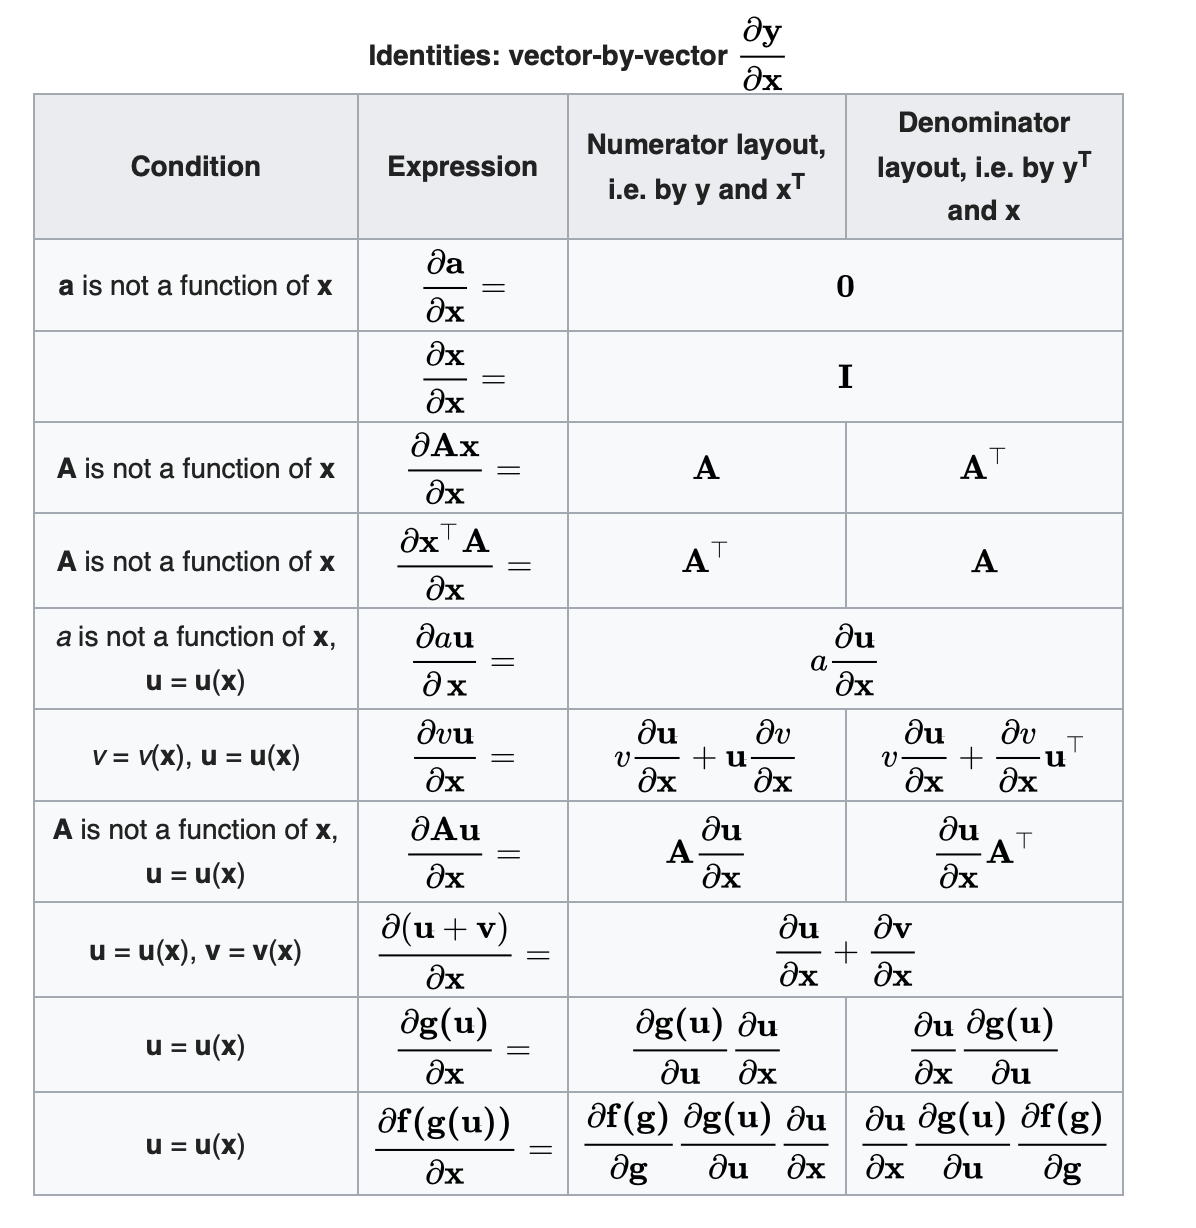
\includegraphics[scale=0.25]{vector_by_vector.png}
    \caption{Denominator layout means $x\in\mathbb{R}^{n\times 1}$}
    \label{}
\end{figure}\end{center}

\begin{equation}
    \begin{aligned}
        \frac{\partial u}{\partial x^T}&=(\frac{\partial u^T}{\partial x})^T\\
        \frac{\partial u^Tv}{\partial x}&=\frac{\partial u^T}{\partial x}v+\frac{\partial v^T}{\partial x}u^T\\
        \frac{\partial uv^T}{\partial x}&=\frac{\partial u}{\partial x}v^T+u\frac{\partial v^T}{\partial x}\\
        \frac{\partial x^Tx}{\partial x}&=2x\\
        \frac{\partial x^TAx}{\partial x}&=(A+A^T)x\\
    \end{aligned}
    \nonumber
\end{equation}
where $x,u,v\in \mathbb{R}^{n\times 1}$

$\textbf{Note:}$ $$\frac{d\|Aw-b\|^2}{dw}
=\frac{d(Aw-b)^T(Aw-b)}{dw}
\\=\frac{d(Aw-b)^T}{dw}(Aw-b)+\frac{d(Aw-b)^T}{dw}(Aw-b)
\\=2A^T(Aw-b)$$

Matrix by vector:
\begin{equation}
    \begin{aligned}
        \frac{\partial AB}{\partial x}&=\frac{\partial A}{\partial x}B+A\frac{\partial B}{\partial x}
    \end{aligned}
    \nonumber
\end{equation}

Matrix by matrix:
\begin{equation}
    \begin{aligned}
        \frac{\partial u^TXv}{\partial X}&=uv^T\\
        \frac{\partial u^TX^TXu}{\partial X}&=2Xuu^T\\
        \frac{\partial [(Xu-v)^T(Xu-v)]}{\partial X}&=2(Xu-v)u^T\\
    \end{aligned}
    \nonumber
\end{equation}

Trace:
\begin{equation}
    \begin{aligned}
        tr(a)&=a\\
        tr(AB)&=tr(BA)\\
        tr(ABC)=&tr(CAB)=tr(BCA)\\
        \frac{\partial tr(AB)}{\partial A}&=B^T\\
        tr(A)&=tr(A^T)\\
        \frac{\partial tr(ABA^TC)}{\partial A}&=CAB+C^TAB^T
    \end{aligned}
    \nonumber
\end{equation}

\section{Matrix Inversion}
\subsection{Woodbury matrix identity}
$${\displaystyle \left(A+UCV\right)^{-1}=A^{-1}-A^{-1}U\left(C^{-1}+VA^{-1}U\right)^{-1}VA^{-1},}$$
where $A, U, C$ and $V$ are conformable matrices: $A$ is $n\times n$, $C$ is $k\times k$, $U$ is $n\times k$, and $V$ is $k\times n$. This can be derived using blockwise matrix inversion.

\underline{Blockwise inversion: }$$
{\displaystyle {\begin{bmatrix}\mathbf {A} &\mathbf {B} \\\mathbf {C} &\mathbf {D} \end{bmatrix}}^{-1}={\begin{bmatrix}\mathbf {A} ^{-1}+\mathbf {A} ^{-1}\mathbf {B} \left(\mathbf {D} -\mathbf {CA} ^{-1}\mathbf {B} \right)^{-1}\mathbf {CA} ^{-1}&-\mathbf {A} ^{-1}\mathbf {B} \left(\mathbf {D} -\mathbf {CA} ^{-1}\mathbf {B} \right)^{-1}\\-\left(\mathbf {D} -\mathbf {CA} ^{-1}\mathbf {B} \right)^{-1}\mathbf {CA} ^{-1}&\left(\mathbf {D} -\mathbf {CA} ^{-1}\mathbf {B} \right)^{-1}\end{bmatrix}}}
$$







\section{Linear Regression: Least Square}
$\textbf{Minimize}_w \mathcal{R}(w)=\|Xw-y\|^2$
\subsection{Normal Equations}
$$\nabla_w\|Xw-y\|^2=2X^T(Xw-y)=0$$
$$\Rightarrow X^TXw=X^Ty$$
These are called the \textbf{normal equations}.
\begin{proposition}
    $\hat{w}$ satisfies $\mathcal{R}(\hat{w})=\min_w\mathcal{R}(w)$ if and only if $\hat{w}$ satisfies the normal equations. (i.e. prove its is the global minimum)
\end{proposition}
\begin{proof}
Consider $\boldsymbol{w}$ with $\boldsymbol{X}^{\top} \boldsymbol{X} \boldsymbol{w}=\boldsymbol{X}^{\top} \boldsymbol{y}$, and any $\boldsymbol{w}^{\prime}$; then $$\begin{aligned}\left\|\boldsymbol{X} \boldsymbol{w}^{\prime}-\boldsymbol{y}\right\|^{2} &=\left\|\boldsymbol{X} \boldsymbol{w}^{\prime}-\boldsymbol{X} \boldsymbol{w}+\boldsymbol{X} \boldsymbol{w}-\boldsymbol{y}\right\|^{2} \\ &=\left\|\boldsymbol{X} \boldsymbol{w}^{\prime}-\boldsymbol{X} \boldsymbol{w}\right\|^{2}+2\left(\boldsymbol{X} \boldsymbol{w}^{\prime}-\boldsymbol{X} \boldsymbol{w}\right)^{\top}(\boldsymbol{X} \boldsymbol{w}-\boldsymbol{y})+\|\boldsymbol{X} \boldsymbol{w}-\boldsymbol{y}\|^{2} \end{aligned}$$
Since
$$
\left(\boldsymbol{X} \boldsymbol{w}^{\prime}-\boldsymbol{X} \boldsymbol{w}\right)^{\top}(\boldsymbol{X} \boldsymbol{w}-\boldsymbol{y})=\left(\boldsymbol{w}^{\prime}-\boldsymbol{w}\right)^{\top}\left(\boldsymbol{X}^{\top} \boldsymbol{X} \boldsymbol{w}-\boldsymbol{X}^{\top} \boldsymbol{y}\right)=0
$$
then
$$
\left\|\boldsymbol{X} \boldsymbol{w}^{\prime}-\boldsymbol{y}\right\|^{2}=\left\|\boldsymbol{X} \boldsymbol{w}^{\prime}-\boldsymbol{X} \boldsymbol{w}\right\|^{2}+\|\boldsymbol{X} \boldsymbol{w}-\boldsymbol{y}\|^{2} \geq\|\boldsymbol{X} \boldsymbol{w}-\boldsymbol{y}\|^{2}
$$
\end{proof}

\section{LU Decomposition (Restricted to Square)}
Triangular matrix saves time when computing $Ax=b$.

Let A be a square matrix. An LU factorization refers to the factorization of A, with proper row and/or column orderings or permutations, into two factors - a lower triangular matrix L and an upper triangular matrix U:

${\displaystyle A=LU.}$
In the lower triangular matrix all elements above the diagonal are zero, in the upper triangular matrix, all the elements below the diagonal are zero. For example, for a $3 \times 3$ matrix $A$, its LU decomposition looks like this:

$${\displaystyle {\begin{bmatrix}a_{11}&a_{12}&a_{13}\\a_{21}&a_{22}&a_{23}\\a_{31}&a_{32}&a_{33}\end{bmatrix}}={\begin{bmatrix}\ell _{11}&0&0\\\ell _{21}&\ell _{22}&0\\\ell _{31}&\ell _{32}&\ell _{33}\end{bmatrix}}{\begin{bmatrix}u_{11}&u_{12}&u_{13}\\0&u_{22}&u_{23}\\0&0&u_{33}\end{bmatrix}}.}$$

$$A=PLU$$
$P$ is a permutation matrix (used to swap row, only one $1$ in every row). $P$ is orthogonal, so $P^{-1}=P^T$.

Solve $Ax=b$:
\begin{equation}
    \begin{aligned}
        Ax&=b\\
        PLUx&=b\\
        \text{Let }y=Ux,&\text{ then solve PLy=b}\\
        Ly&=P^Tb
    \end{aligned}
    \nonumber
\end{equation}
Complexity: $O(n^3)$

\section{SVD: Singular Value Decomposition}
For a $n\times m$ matrix $A$ with rank $r$,
\begin{equation}
    \begin{aligned}
        A_{n\times m}=&U_{n\times n}\Sigma_{n\times m}V^T_{m\times m}\\
        &=\sum_{i=1}^rs_iu_iv_i^T\\
        &=\begin{bmatrix}
            \vline&\vline&\cdots&\vline\\
            u_1&u_2&\cdots&u_n\\
            \vline&\vline&\cdots&\vline
        \end{bmatrix}\begin{bmatrix}
            s_1&&&&&&\\
            &s_2&&&&&\\
            &&\ddots&&&&\\
            &&&s_r&&&\\
            &&&&0&&\\
            &&&&&\ddots&\\
            &&&&&&0
        \end{bmatrix}\begin{bmatrix}
            \vline&\vline&\cdots&\vline\\
            v_1&v_2&\cdots&v_m\\
            \vline&\vline&\cdots&\vline
        \end{bmatrix}^T
    \end{aligned}
    \nonumber
\end{equation}
$U,V$ are orthogonal matrices. $u_i\in \mathbb{R}^{n\times 1}$ are left singular vectors, $v_i\in \mathbb{R}^{m\times 1}$ are right singular vectors. $s_i,i=1,...,r$ are singular values (absolute values of eigenvalues of a normal matrix).

Complexity:$O(mn^2+n^3)$


\subsection{Pseudo-inverse}
We can't compute the inverse matrix of a singular matrix. We can use pseudo-inverse matrix.
$$A^+_{m\times n}=\sum_{i=1}^r\frac{1}{s_i}v_iu_i^T=V\Sigma^+U^T$$
Where $$\Sigma^+=\begin{bmatrix}
    \frac{1}{s_1}&&&&&&\\
    &\frac{1}{s_2}&&&&&\\
    &&\ddots&&&&\\
    &&&\frac{1}{s_r}&&&\\
    &&&&0&&\\
    &&&&&\ddots&\\
    &&&&&&0
\end{bmatrix}$$
The SVD may not be unique, but the pseudo-inverse of $A$, $A^+$ is unique.
\begin{equation}
    \begin{aligned}
        AA^+&=\sum_{i=1}^ru_iu_i^T=\begin{bmatrix}
            I_{r\times r}&	O_{r\times n-r}\\
            O_{n-r\times r}&	O_{n-r\times n-r}
        \end{bmatrix}_{n\times n}\\
        A^+A&=\sum_{i=1}^rv_iv_i^T=\begin{bmatrix}
            I_{r\times r}&	O_{r\times m-r}\\
            O_{m-r\times r}&	O_{m-r\times m-r}
        \end{bmatrix}_{m\times m}
    \end{aligned}
    \nonumber
\end{equation}
If $A^{-1}$ exists, $A^{-1}=A^+$.

\subsection{Analysis of $A^TA$ and $AA^T$}
\begin{equation}
    \begin{aligned}
        A^TA&=(U\Sigma V^T)^T(U\Sigma V^T)\\
        &=V\Sigma^TU^TU\Sigma V^T\\
        &=V\Sigma^T\Sigma V^T\\
        &=V\Sigma^2 V^T\\
        \Rightarrow	V&=A^TU\Sigma^+
    \end{aligned}
    \nonumber
\end{equation}
Columns of $V$ are the eigenvectors of $A^TA$.

The diagonal entries of $\Sigma^2$, $s_1^2,s_2^2,...,s_r^2$ are the eigenvalues of $A^TA$.

Similarly: $$AA^T=U\Sigma^2U^T$$
$$\Rightarrow U=AV\Sigma^+$$
Columns of $U$ are the eigenvectors of $AA^T$.

\textbf{Fact:} $A^TA$ is positive semi-definite.

\subsection{Solve Normal Equations}
Solve $X^TXw=X^Ty$, $$\hat{w}_{ols}=X^+y$$
$$X^TX\hat{w}_{ols}=X^TXX^+y=(X^T(XX^+))y=X^Ty$$

\subsection{Low-Rank Approximation}
For a $n\times m$ matrix $A$ with rank $r$, $A=\sum_{i=1}^rs_iu_iv_u^T$.

\textbf{Rank-$k$ approximation} for $A$ is
$$A_k=\sum_{i=1}^ks_iu_iv_u^T$$
Where $s_1\geq s_2\geq \cdots\geq 0$




\begin{thebibliography}{1}
    \bibitem{Long2015Fully}  MATH 417: Christopher J Leininger  \newblock Introduction to Abstract Algebra (Draft)  2017.
    \bibitem{Long2015Fully} MATH 484
    \bibitem{Long2015Fully} ECE 490
    \bibitem{Long2015Fully} STAT 425
    \bibitem{Long2015Fully} CS/MATH 357
\end{thebibliography}


\end{document}
\bibliography{reference}
\bibliographystyle{unsrt}